We compute the ground state of the TFI model \eqref{eq:TFI_Hamiltonian} using disoTPS and TEBD with imaginary time $\tau = -i t$. As initial state we choose the product state $|\Psi_i\rangle=|\uparrow\rangle\otimes\cdots\otimes|\uparrow\rangle$ of all spins pointing up. One can expand the initial state in terms of energy eigenstates
\begin{equation}
	|\Psi_i\rangle = \sum_{n} \Psi_n |n\rangle.
\end{equation}
Applying the time evolution and normalizing then leads to the state
\begin{equation}
	|\Psi(t)\rangle = e^{-i\tau\hat{H}} |\Psi_i\rangle = \frac{1}{\mathcal{N}} \sum_{n} \Psi_n e^{-iE_n\tau} |n\rangle = \frac{1}{\mathcal{N}} \sum_{n} \Psi_n e^{-E_nt} |n\rangle
\end{equation}
with
\begin{equation}
	\mathcal{N} = \left\lVert\sum_{n} \Psi_n e^{-E_nt}\right\rVert
\end{equation}
If we now take the limit $t \rightarrow \infty$ and assume that the ground state $|0\rangle$ with the lowest energy $E_0$ is nondegenerate, all states except the ground state vanish because of the exponential terms $e^{-E_nt}$. We end up with the ground state
\begin{equation}
	|\Psi(t\rightarrow\infty)\rangle = |0\rangle.
\end{equation}
To use the TEBD algorithm we must choose a good step size $\Delta t$. The total error of a single TEBD step evolving the disoTPS by (imaginary) time $\Delta t$ is a sum of three errors,
\begin{equation}
	\varepsilon_\text{TEBD} = \varepsilon_\text{Trotter} + \varepsilon_\text{trunc} + \varepsilon_{\text{YB}}.
\end{equation} 
The trotterization error $\varepsilon_\text{Trotter}$ comes from the Suzuki-Trotter decomposition, the truncation error $\varepsilon_\text{trunc}$ from locally applying the bond operators, and the YB error $\varepsilon_{\text{YB}}$ gets introduced when shifting the orthogonality hypersurface. A smaller time step $\Delta t$ decreases both $\varepsilon_\text{Trotter}$ and $\varepsilon_\text{trunc}$ while the YB error $\varepsilon_{\text{YB}}$ is not directly affected. However, since for a smaller time step $\Delta t$ more TEBD iterations are necessary to approach the limit $t\rightarrow\infty$, YB errors add up and prevent the state from reaching the true ground state. Therefore we expect, similar to \cite{cite:isometric_tensor_network_states_in_two_dimensions, cite:efficient_simulation_of_dynamics_in_two_dimensional_quantum_spin_systems}, that the YB-error dominates for small time steps, while the trotterization and truncation errors dominate for larger time steps. The best results can be achieved when the time step $\Delta t$ is tuned such that $\varepsilon_\text{Trotter} + \varepsilon_\text{trunc} \approx \varepsilon_{\text{YB}}$. \par
In figure \figref{} we benchmark the different algorithms for the YB move that were discussed in section \ref{sec:disoTPS_yang_baxter_move}. We perform an imaginary time evolution of the TFI model with a transverse field of $g = 3.5$, using second order TEBD and time steps $\Delta t \in \left[0.02, 0.5\right]$. The model is put on a $4\times4$ square lattice containing $32$ spins. For each data point we start at $\Delta t = 0.5$, slowly decreasing the time step until arriving at the desired time step $\Delta t$. We then perform another $50$ TEBD iterations and compute the average energy of the last 20 iterations. We then compute the relative error compared to the numerically exact DMRG reference simulation with a bond dimension of $\chi = 1024$ and plot the error against the time step $\Delta t$. \par
For figure \figref{}(a) we used a simple SVD for the YB move. The resulting error is large and the ground state energy is only found up to an accuracy of $10^{-3}$. If we use the initialization discussed in appendix \ref{} as a guess for the disentangling unitary, the ground state estimate improves by half an order of magnitude, see \figref{}(b). Using the Evenbly-Vidal algorithm for the YB move as discussed in section \ref{sec:YB_move_iterative_local_optimization} results in a comparable error, see \figref{}(c). In \figref{}(d) we used the Evenbly-Vidal algorithm for disentangling, optimizing the Rényi entropy with $\alpha = 2$. This improves the results drastically, pushing the relative error down to $10^{-5}$. Figures \figref{}(e)-(h) show the results when disentangling by optimizing the truncation error using Riemannian optimization. This performs slightly worse than when optimizing the Renyi-entropy. The reason for this is the following: While minimizing the truncation error leads to a better local YB-move it can lead to a larger error for the following YB-moves on the column. \todo{besser formulieren}. Conjugate Gradients (CG) and the Trust Region Method (TRM) perform similarly. Notably, the approximate version of both algorithms performs almost as good as the exact version while being much faster. Finally in figures \ref{}(i-l) we show the YB move with disentangling optimizing the Rényi entropy with $\alpha = 1/2$. Out of all methods tested this obtains the most accurate results. The TRM is able to achieve a slightly lower error than CG. We again observe that the approximate versions of both CG and TRM perform as well as the exact algorithms. \par
To conclude, we find that disentangling while optimizing the Rényi $\alpha=1/2$ entropy with the approximate TRM is the best method out of the methods tested. We will therefore use this method for the following plots. \par
\begin{figure}
	\centering
	\begin{minipage}{1.0\textwidth}
		\centering
		\begin{tikzpicture}[scale=1, trim axis left, trim axis right]
			\begin{axis}[ylabel={$\Delta E / E_\text{exact}$}, grid=both, grid style={gray!20}, every axis plot/.append style={very thick}, scale only axis, height=\gsEnergyVsDtauFigureHeight, width=\gsEnergyVsDtauFigureWidth, xmode=log, ymode=log, ymin=1e-6, ymax=1e-1, legend style={nodes={scale=\legendscale, transform shape, font=\small}}, legend pos=south west, title={\footnotesize\textbf{SVD}}, xticklabels={}, legend cell align={left}]
				%	
				\addplot[color = 3blue1, mark=*]
				table[x=dtau, y=delta_E_D_max_2, col sep=space]{figures/plots/TFI/gs_energy_vs_dtau/data/gs_energy_vs_dtau_square_svd.txt};
				\addlegendentry{$D = 2$}
				%	
				\addplot[color = 3blue2, mark=*]
				table[x=dtau, y=delta_E_D_max_4, col sep=space]{figures/plots/TFI/gs_energy_vs_dtau/data/gs_energy_vs_dtau_square_svd.txt};
				\addlegendentry{$D = 4$}
				%	
				\addplot[color = 3blue3, mark=*]
				table[x=dtau, y=delta_E_D_max_6, col sep=space]{figures/plots/TFI/gs_energy_vs_dtau/data/gs_energy_vs_dtau_square_svd.txt};
				\addlegendentry{$D = 6$}
			\end{axis}%
		\end{tikzpicture}%
		\,\,
		\begin{tikzpicture}[scale=1, trim axis left, trim axis right]
			\begin{axis}[grid=both, grid style={gray!20}, every axis plot/.append style={very thick}, scale only axis, height=\gsEnergyVsDtauFigureHeight, width=\gsEnergyVsDtauFigureWidth, xmode=log, ymode=log, ymin=1e-6, ymax=1e-1, yticklabels={}, title={\footnotesize\textbf{SVD + init}}, xticklabels={}]
				%	
				\addplot[color = 3blue1, mark=*]
				table[x=dtau, y=delta_E_D_max_2, col sep=space]{figures/plots/TFI/gs_energy_vs_dtau/data/gs_energy_vs_dtau_square_svd_init_polar.txt};
				%\addlegendentry{$D = 2$}
				%	
				\addplot[color = 3blue2, mark=*]
				table[x=dtau, y=delta_E_D_max_4, col sep=space]{figures/plots/TFI/gs_energy_vs_dtau/data/gs_energy_vs_dtau_square_svd_init_polar.txt};
				%\addlegendentry{$D = 4$}
				%	
				\addplot[color = 3blue3, mark=*]
				table[x=dtau, y=delta_E_D_max_6, col sep=space]{figures/plots/TFI/gs_energy_vs_dtau/data/gs_energy_vs_dtau_square_svd_init_polar.txt};
				%\addlegendentry{$D = 6$}
			\end{axis}%
		\end{tikzpicture}%
		\,\,
		\begin{tikzpicture}[scale=1, trim axis left, trim axis right]
			\begin{axis}[grid=both, grid style={gray!20}, every axis plot/.append style={very thick}, scale only axis, height=\gsEnergyVsDtauFigureHeight, width=\gsEnergyVsDtauFigureWidth, xmode=log, ymode=log, ymin=1e-6, ymax=1e-1, yticklabels={}, title={\footnotesize\textbf{EV trunc}}, xticklabels={}]
				%	
				\addplot[color = 3blue1, mark=*]
				table[x=dtau, y=delta_E_D_max_2, col sep=space]{figures/plots/TFI/gs_energy_vs_dtau/data/gs_energy_vs_dtau_square_iterate_polar.txt};
				%\addlegendentry{$D = 2$}
				%	
				\addplot[color = 3blue2, mark=*]
				table[x=dtau, y=delta_E_D_max_4, col sep=space]{figures/plots/TFI/gs_energy_vs_dtau/data/gs_energy_vs_dtau_square_iterate_polar.txt};
				%\addlegendentry{$D = 4$}
				%	
				\addplot[color = 3blue3, mark=*]
				table[x=dtau, y=delta_E_D_max_6, col sep=space]{figures/plots/TFI/gs_energy_vs_dtau/data/gs_energy_vs_dtau_square_iterate_polar.txt};
				%\addlegendentry{$D = 6$}
			\end{axis}%
		\end{tikzpicture}%
		\,\,
		\begin{tikzpicture}[scale=1, trim axis left, trim axis right]
			\begin{axis}[grid=both, grid style={gray!20}, every axis plot/.append style={very thick}, scale only axis, height=\gsEnergyVsDtauFigureHeight, width=\gsEnergyVsDtauFigureWidth, xmode=log, ymode=log, ymin=1e-6, ymax=1e-1, yticklabels={}, title={\footnotesize\textbf{EV Rényi-2}}, xticklabels={}]
				%	
				\addplot[color = 3blue1, mark=*]
				table[x=dtau, y=delta_E_D_max_2, col sep=space]{figures/plots/TFI/gs_energy_vs_dtau/data/gs_energy_vs_dtau_square_svd_disent_renyi_2.0_power_iteration.txt};
				%\addlegendentry{$D = 2$}
				%	
				\addplot[color = 3blue2, mark=*]
				table[x=dtau, y=delta_E_D_max_4, col sep=space]{figures/plots/TFI/gs_energy_vs_dtau/data/gs_energy_vs_dtau_square_svd_disent_renyi_2.0_power_iteration.txt};
				%\addlegendentry{$D = 4$}
				%	
				\addplot[color = 3blue3, mark=*]
				table[x=dtau, y=delta_E_D_max_6, col sep=space]{figures/plots/TFI/gs_energy_vs_dtau/data/gs_energy_vs_dtau_square_svd_disent_renyi_2.0_power_iteration.txt};
				%\addlegendentry{$D = 6$}
			\end{axis}%
		\end{tikzpicture}%
	\end{minipage}
	\begin{minipage}{1.0\textwidth}
		\centering%
		% ====================================================================================
		% 2nd line
		% ====================================================================================
		\begin{tikzpicture}[scale=1, trim axis left, trim axis right]
			\begin{axis}[ylabel={$\Delta E / E_\text{exact}$}, grid=both, grid style={gray!20}, every axis plot/.append style={very thick}, scale only axis, height=\gsEnergyVsDtauFigureHeight, width=\gsEnergyVsDtauFigureWidth, xmode=log, ymode=log, ymin=1e-6, ymax=1e-1, title={\footnotesize\textbf{CG trunc}}, xticklabels={}]
				%	
				\addplot[color = 3blue1, mark=*]
				table[x=dtau, y=delta_E_D_max_2, col sep=space]{figures/plots/TFI/gs_energy_vs_dtau/data/gs_energy_vs_dtau_square_svd_disent_trunc_error_cg.txt};
				%\addlegendentry{$D = 2$}
				%	
				\addplot[color = 3blue2, mark=*]
				table[x=dtau, y=delta_E_D_max_4, col sep=space]{figures/plots/TFI/gs_energy_vs_dtau/data/gs_energy_vs_dtau_square_svd_disent_trunc_error_cg.txt};
				%\addlegendentry{$D = 4$}
				%	
				\addplot[color = 3blue3, mark=*]
				table[x=dtau, y=delta_E_D_max_6, col sep=space]{figures/plots/TFI/gs_energy_vs_dtau/data/gs_energy_vs_dtau_square_svd_disent_trunc_error_cg.txt};
				%\addlegendentry{$D = 6$}
			\end{axis}%
		\end{tikzpicture}%
		\,\,
		\begin{tikzpicture}[scale=1, trim axis left, trim axis right]
			\begin{axis}[grid=both, grid style={gray!20}, every axis plot/.append style={very thick}, scale only axis, height=\gsEnergyVsDtauFigureHeight, width=\gsEnergyVsDtauFigureWidth, xmode=log, ymode=log, ymin=1e-6, ymax=1e-1, yticklabels={}, title={\footnotesize\textbf{approx CG trunc}}, xticklabels={}]
				%	
				\addplot[color = 3blue1, mark=*]
				table[x=dtau, y=delta_E_D_max_2, col sep=space]{figures/plots/TFI/gs_energy_vs_dtau/data/gs_energy_vs_dtau_square_svd_disent_trunc_error_approx_cg.txt};
				%\addlegendentry{$D = 2$}
				%	
				\addplot[color = 3blue2, mark=*]
				table[x=dtau, y=delta_E_D_max_4, col sep=space]{figures/plots/TFI/gs_energy_vs_dtau/data/gs_energy_vs_dtau_square_svd_disent_trunc_error_approx_cg.txt};
				%\addlegendentry{$D = 4$}
				%	
				\addplot[color = 3blue3, mark=*]
				table[x=dtau, y=delta_E_D_max_6, col sep=space]{figures/plots/TFI/gs_energy_vs_dtau/data/gs_energy_vs_dtau_square_svd_disent_trunc_error_approx_cg.txt};
				%\addlegendentry{$D = 6$}
			\end{axis}%
		\end{tikzpicture}%
		\,\,
		\begin{tikzpicture}[scale=1, trim axis left, trim axis right]
			\begin{axis}[grid=both, grid style={gray!20}, every axis plot/.append style={very thick}, scale only axis, height=\gsEnergyVsDtauFigureHeight, width=\gsEnergyVsDtauFigureWidth, xmode=log, ymode=log, ymin=1e-6, ymax=1e-1, yticklabels={}, title={\footnotesize\textbf{TRM trunc}}, xticklabels={}]
				%	
				\addplot[color = 3blue1, mark=*]
				table[x=dtau, y=delta_E_D_max_2, col sep=space]{figures/plots/TFI/gs_energy_vs_dtau/data/gs_energy_vs_dtau_square_svd_disent_trunc_error_trm.txt};
				%\addlegendentry{$D = 2$}
				%	
				\addplot[color = 3blue2, mark=*]
				table[x=dtau, y=delta_E_D_max_4, col sep=space]{figures/plots/TFI/gs_energy_vs_dtau/data/gs_energy_vs_dtau_square_svd_disent_trunc_error_trm.txt};
				%\addlegendentry{$D = 4$}
				%	
				\addplot[color = 3blue3, mark=*]
				table[x=dtau, y=delta_E_D_max_6, col sep=space]{figures/plots/TFI/gs_energy_vs_dtau/data/gs_energy_vs_dtau_square_svd_disent_trunc_error_trm.txt};
				%\addlegendentry{$D = 6$}
			\end{axis}%
		\end{tikzpicture}%
		\,\,
		\begin{tikzpicture}[scale=1, trim axis left, trim axis right]
			\begin{axis}[grid=both, grid style={gray!20}, every axis plot/.append style={very thick}, scale only axis, height=\gsEnergyVsDtauFigureHeight, width=\gsEnergyVsDtauFigureWidth, xmode=log, ymode=log, ymin=1e-6, ymax=1e-1, yticklabels={}, title={\footnotesize\textbf{approx TRM trunc}}, xticklabels={}]
				%	
				\addplot[color = 3blue1, mark=*]
				table[x=dtau, y=delta_E_D_max_2, col sep=space]{figures/plots/TFI/gs_energy_vs_dtau/data/gs_energy_vs_dtau_square_svd_disent_trunc_error_approx_trm.txt};
				%\addlegendentry{$D = 2$}
				%	
				\addplot[color = 3blue2, mark=*]
				table[x=dtau, y=delta_E_D_max_4, col sep=space]{figures/plots/TFI/gs_energy_vs_dtau/data/gs_energy_vs_dtau_square_svd_disent_trunc_error_approx_trm.txt};
				%\addlegendentry{$D = 4$}
				%	
				\addplot[color = 3blue3, mark=*]
				table[x=dtau, y=delta_E_D_max_6, col sep=space]{figures/plots/TFI/gs_energy_vs_dtau/data/gs_energy_vs_dtau_square_svd_disent_trunc_error_approx_trm.txt};
				%\addlegendentry{$D = 6$}
			\end{axis}%
		\end{tikzpicture}%
	\end{minipage}
	\begin{minipage}{1.0\textwidth}
		\centering%
		% ====================================================================================
		% 3rd line
		% ====================================================================================
		\begin{tikzpicture}[scale=1, trim axis left, trim axis right]
			\begin{axis}[xlabel=$\Delta\tau$, ylabel={$\Delta E / E_\text{exact}$}, grid=both, grid style={gray!20}, every axis plot/.append style={very thick}, scale only axis, height=\gsEnergyVsDtauFigureHeight, width=\gsEnergyVsDtauFigureWidth, xmode=log, ymode=log, ymin=1e-6, ymax=1e-1, title={\footnotesize\textbf{CG Rényi-0.5}}]
				%	
				\addplot[color = 3blue1, mark=*]
				table[x=dtau, y=delta_E_D_max_2, col sep=space]{figures/plots/TFI/gs_energy_vs_dtau/data/gs_energy_vs_dtau_square_svd_disent_renyi_0.5_cg.txt};
				%\addlegendentry{$D = 2$}
				%	
				\addplot[color = 3blue2, mark=*]
				table[x=dtau, y=delta_E_D_max_4, col sep=space]{figures/plots/TFI/gs_energy_vs_dtau/data/gs_energy_vs_dtau_square_svd_disent_renyi_0.5_cg.txt};
				%\addlegendentry{$D = 4$}
				%	
				\addplot[color = 3blue3, mark=*]
				table[x=dtau, y=delta_E_D_max_6, col sep=space]{figures/plots/TFI/gs_energy_vs_dtau/data/gs_energy_vs_dtau_square_svd_disent_renyi_0.5_cg.txt};
				%\addlegendentry{$D = 6$}
			\end{axis}%
		\end{tikzpicture}%
		\,\,
		\begin{tikzpicture}[scale=1, trim axis left, trim axis right]
			\begin{axis}[xlabel=$\Delta\tau$, grid=both, grid style={gray!20}, every axis plot/.append style={very thick}, scale only axis, height=\gsEnergyVsDtauFigureHeight, width=\gsEnergyVsDtauFigureWidth, xmode=log, ymode=log, ymin=1e-6, ymax=1e-1, yticklabels={}, title={\footnotesize\textbf{appr.\,CG\,Rényi-0.5}}]
				%	
				\addplot[color = 3blue1, mark=*]
				table[x=dtau, y=delta_E_D_max_2, col sep=space]{figures/plots/TFI/gs_energy_vs_dtau/data/gs_energy_vs_dtau_square_svd_disent_renyi_0.5_approx_cg.txt};
				%\addlegendentry{$D = 2$}
				%	
				\addplot[color = 3blue2, mark=*]
				table[x=dtau, y=delta_E_D_max_4, col sep=space]{figures/plots/TFI/gs_energy_vs_dtau/data/gs_energy_vs_dtau_square_svd_disent_renyi_0.5_approx_cg.txt};
				%\addlegendentry{$D = 4$}
				%	
				\addplot[color = 3blue3, mark=*]
				table[x=dtau, y=delta_E_D_max_6, col sep=space]{figures/plots/TFI/gs_energy_vs_dtau/data/gs_energy_vs_dtau_square_svd_disent_renyi_0.5_approx_cg.txt};
				%\addlegendentry{$D = 6$}
			\end{axis}%
		\end{tikzpicture}%
		\,\,
		\begin{tikzpicture}[scale=1, trim axis left, trim axis right]
			\begin{axis}[xlabel=$\Delta\tau$, grid=both, grid style={gray!20}, every axis plot/.append style={very thick}, scale only axis, height=\gsEnergyVsDtauFigureHeight, width=\gsEnergyVsDtauFigureWidth, xmode=log, ymode=log, ymin=1e-6, ymax=1e-1, yticklabels={}, title={\footnotesize\textbf{TRM\,Rényi-0.5}}]
				%	
				\addplot[color = 3blue1, mark=*]
				table[x=dtau, y=delta_E_D_max_2, col sep=space]{figures/plots/TFI/gs_energy_vs_dtau/data/gs_energy_vs_dtau_square_svd_disent_renyi_0.5_trm.txt};
				%\addlegendentry{$D = 2$}
				%	
				\addplot[color = 3blue2, mark=*]
				table[x=dtau, y=delta_E_D_max_4, col sep=space]{figures/plots/TFI/gs_energy_vs_dtau/data/gs_energy_vs_dtau_square_svd_disent_renyi_0.5_trm.txt};
				%\addlegendentry{$D = 4$}
				%	
				\addplot[color = 3blue3, mark=*]
				table[x=dtau, y=delta_E_D_max_6, col sep=space]{figures/plots/TFI/gs_energy_vs_dtau/data/gs_energy_vs_dtau_square_svd_disent_renyi_0.5_trm.txt};
				%\addlegendentry{$D = 6$}
			\end{axis}%
		\end{tikzpicture}%
		\,\,
		\begin{tikzpicture}[scale=1, trim axis left, trim axis right]
			\begin{axis}[xlabel=$\Delta\tau$, grid=both, grid style={gray!20}, every axis plot/.append style={very thick}, scale only axis, height=\gsEnergyVsDtauFigureHeight, width=\gsEnergyVsDtauFigureWidth, xmode=log, ymode=log, ymin=1e-6, ymax=1e-1, yticklabels={}, title={\footnotesize\textbf{appr.\,TRM\,Rényi-0.5}}]
				%	
				\addplot[color = 3blue1, mark=*]
				table[x=dtau, y=delta_E_D_max_2, col sep=space]{figures/plots/TFI/gs_energy_vs_dtau/data/gs_energy_vs_dtau_square_svd_disent_renyi_0.5_approx_trm.txt};
				%\addlegendentry{$D = 2$}
				%	
				\addplot[color = 3blue2, mark=*]
				table[x=dtau, y=delta_E_D_max_4, col sep=space]{figures/plots/TFI/gs_energy_vs_dtau/data/gs_energy_vs_dtau_square_svd_disent_renyi_0.5_approx_trm.txt};
				%\addlegendentry{$D = 4$}
				%	
				\addplot[color = 3blue3, mark=*]
				table[x=dtau, y=delta_E_D_max_6, col sep=space]{figures/plots/TFI/gs_energy_vs_dtau/data/gs_energy_vs_dtau_square_svd_disent_renyi_0.5_approx_trm.txt};
				%\addlegendentry{$D = 6$}
			\end{axis}%
		\end{tikzpicture}%
	\end{minipage}
	\caption{We benchmark the different implemented methods for the YB move on the TFI model on a $4\times4$ square lattice. The transverse field is set to $g = 3.5$. We compute the ground state energy with imaginary TEBD for different time step sizes $\Delta\tau$. First row: SVD splitting without disentangling, SVD splitting with a disentangling unitary initialized with an SVD as in \cite{cite:isometric_tensor_network_states_in_two_dimensions, cite:efficient_simulation_of_dynamics_in_two_dimensional_quantum_spin_systems}, Evenbly-Vidal minimization of the truncation error, and Evenbly-Vidal minimization of the Rényi-2 entropy. Second row: Disentangling with Riemannian optimization of the truncation error. Third row: Disentangling with Riemannian optimization of the  Rényi-1/2 entropy. All iterative methods were run for a maximum of $N_\text{iter} = 100$ iterations per YB move. The bond dimension of the orthogonality hypersurface was set to $\chi = 6\cdot D$.}
	\label{fig:tfi_gs_energy_vs_dtau_different_methods}
\end{figure}
It is also interesting to observe how many iterations of optimization are necessary for the disentangling to converge. In figure \figref{} we compare different values for the maximum number of iterations $N_\text{iters} = 50, 100, 200$. We observe that already for $N_\text{iters} = 50$ the algorithm is converged. \par
\begin{figure}
	\centering
	\begin{minipage}{1.0\textwidth}
		\centering
		\begin{tikzpicture}[scale=1, trim axis left, trim axis right]
			\begin{axis}[xlabel=$\text{d}\tau$, ylabel={$\Delta E / E_\text{exact}$}, grid=both, grid style={gray!20}, every axis plot/.append style={very thick}, scale only axis, height=\gsEnergyVsDtauFigureHeight, width=\gsEnergyVsDtauFigureWidth, xmode=log, ymode=log, ymin=1e-6, ymax=1e-1, title={$N_\text{iters} = 1$}]
				%	
				\addplot[color = 3blue1, mark=*]
				table[x=dtau, y=delta_E_D_max_2, col sep=space]{figures/plots/TFI/gs_energy_vs_dtau/data/gs_energy_vs_dtau_square_svd_disent_renyi_0.5_approx_trm_N_iters_1.txt};
				%\addlegendentry{$D = 2$}
				%	
				\addplot[color = 3blue2, mark=*]
				table[x=dtau, y=delta_E_D_max_4, col sep=space]{figures/plots/TFI/gs_energy_vs_dtau/data/gs_energy_vs_dtau_square_svd_disent_renyi_0.5_approx_trm_N_iters_1.txt};
				%\addlegendentry{$D = 4$}
				%	
				\addplot[color = 3blue3, mark=*]
				table[x=dtau, y=delta_E_D_max_6, col sep=space]{figures/plots/TFI/gs_energy_vs_dtau/data/gs_energy_vs_dtau_square_svd_disent_renyi_0.5_approx_trm_N_iters_1.txt};
				%\addlegendentry{$D = 6$}
			\end{axis}%
		\end{tikzpicture}%
		\,\,
		\begin{tikzpicture}[scale=1, trim axis left, trim axis right]
			\begin{axis}[xlabel=$\text{d}\tau$, grid=both, grid style={gray!20}, every axis plot/.append style={very thick}, scale only axis, height=\gsEnergyVsDtauFigureHeight, width=\gsEnergyVsDtauFigureWidth, xmode=log, ymode=log, ymin=1e-6, ymax=1e-1, yticklabels={}, title={$N_\text{iters} = 10$}]
				%	
				\addplot[color = 3blue1, mark=*]
				table[x=dtau, y=delta_E_D_max_2, col sep=space]{figures/plots/TFI/gs_energy_vs_dtau/data/gs_energy_vs_dtau_square_svd_disent_renyi_0.5_approx_trm_N_iters_10.txt};
				%\addlegendentry{$D = 2$}
				%	
				\addplot[color = 3blue2, mark=*]
				table[x=dtau, y=delta_E_D_max_4, col sep=space]{figures/plots/TFI/gs_energy_vs_dtau/data/gs_energy_vs_dtau_square_svd_disent_renyi_0.5_approx_trm_N_iters_10.txt};
				%\addlegendentry{$D = 4$}
				%	
				\addplot[color = 3blue3, mark=*]
				table[x=dtau, y=delta_E_D_max_6, col sep=space]{figures/plots/TFI/gs_energy_vs_dtau/data/gs_energy_vs_dtau_square_svd_disent_renyi_0.5_approx_trm_N_iters_10.txt};
				%\addlegendentry{$D = 6$}
			\end{axis}%
		\end{tikzpicture}%
		\,\,
		\begin{tikzpicture}[scale=1, trim axis left, trim axis right]
			\begin{axis}[xlabel=$\text{d}\tau$, grid=both, grid style={gray!20}, every axis plot/.append style={very thick}, scale only axis, height=\gsEnergyVsDtauFigureHeight, width=\gsEnergyVsDtauFigureWidth, xmode=log, ymode=log, ymin=1e-6, ymax=1e-1, yticklabels={}, title={$N_\text{iters} = 50$}]
				%	
				\addplot[color = 3blue1, mark=*]
				table[x=dtau, y=delta_E_D_max_2, col sep=space]{figures/plots/TFI/gs_energy_vs_dtau/data/gs_energy_vs_dtau_square_svd_disent_renyi_0.5_approx_trm_N_iters_50.txt};
				%\addlegendentry{$D = 2$}
				%	
				\addplot[color = 3blue2, mark=*]
				table[x=dtau, y=delta_E_D_max_4, col sep=space]{figures/plots/TFI/gs_energy_vs_dtau/data/gs_energy_vs_dtau_square_svd_disent_renyi_0.5_approx_trm_N_iters_50.txt};
				%\addlegendentry{$D = 4$}
				%	
				\addplot[color = 3blue3, mark=*]
				table[x=dtau, y=delta_E_D_max_6, col sep=space]{figures/plots/TFI/gs_energy_vs_dtau/data/gs_energy_vs_dtau_square_svd_disent_renyi_0.5_approx_trm_N_iters_50.txt};
				%\addlegendentry{$D = 6$}
			\end{axis}%
		\end{tikzpicture}%
		\,\,
		\begin{tikzpicture}[scale=1, trim axis left, trim axis right]
			\begin{axis}[xlabel=$\text{d}\tau$, grid=both, grid style={gray!20}, every axis plot/.append style={very thick}, scale only axis, height=\gsEnergyVsDtauFigureHeight, width=\gsEnergyVsDtauFigureWidth, xmode=log, ymode=log, ymin=1e-6, ymax=1e-1, yticklabels={}, title={$N_\text{iters} = 200$}, legend style={nodes={scale=\legendscale, transform shape}}, legend pos=north west]
				%	
				\addplot[color = 3blue1, mark=*]
				table[x=dtau, y=delta_E_D_max_2, col sep=space]{figures/plots/TFI/gs_energy_vs_dtau/data/gs_energy_vs_dtau_square_svd_disent_renyi_0.5_approx_trm_N_iters_200.txt};
				\addlegendentry{$D = 2$}
				%	
				\addplot[color = 3blue2, mark=*]
				table[x=dtau, y=delta_E_D_max_4, col sep=space]{figures/plots/TFI/gs_energy_vs_dtau/data/gs_energy_vs_dtau_square_svd_disent_renyi_0.5_approx_trm_N_iters_200.txt};
				\addlegendentry{$D = 4$}
				%	
				\addplot[color = 3blue3, mark=*]
				table[x=dtau, y=delta_E_D_max_6, col sep=space]{figures/plots/TFI/gs_energy_vs_dtau/data/gs_energy_vs_dtau_square_svd_disent_renyi_0.5_approx_trm_N_iters_200.txt};
				\addlegendentry{$D = 6$}
			\end{axis}%
		\end{tikzpicture}%
	\end{minipage}
	\caption{In this figure we test how many iterations of Riemannian optimization are necessary for the approximate TRM algorithm minimizing the Rényi-$0.5$ entropy to converge. As a model we use the TFI model on a $4\times4$ suare lattice with a transverse field of $g = 3.5$. The bond dimension of the orthogonality hypersurface is set to $\chi=6\cdot D$. We compute the ground state energy with imaginary TEBD for different time step sizes $\text{d}\tau$.}
	\label{fig:tfi_gs_energy_vs_dtau_different_N_iters}
\end{figure}
As discussed in section \ref{sec:disoTPS_TEBD} both first and second order TEBD require the same number of YB-moves, while second order TEBD leads to a smaller trotterization error $\varepsilon_\text{Trotter}$ and therefore allows us to go to larger time steps $\Delta t$. In figure \figref{} we compare TEBD of first and second order and observe the expected behaviour. The lowest energy is achieved at a smaller timestep compared to TEBD2, and the error of TEBD1 is a magnitude larger than that of TEBD2. \todo{Discuss that maybe the local truncation error increases?}\par
\begin{figure}
	\centering
	\begin{tikzpicture}[scale=1, trim axis left, trim axis right]
		\begin{axis}[xlabel=$\text{d}\tau$, ylabel={$\Delta E / E_\text{exact}$}, grid=both, grid style={gray!20}, every axis plot/.append style={very thick}, scale only axis, height=\gsEnergyVsDtauFigureHeight, width=\gsEnergyVsDtauFigureWidth, xmode=log, ymode=log, ymin=1e-6, ymax=1e-1, title={TEBD1}]
			%	
			\addplot[color = 3blue1, mark=*]
			table[x=dtau, y=delta_E_D_max_2, col sep=space]{figures/plots/TFI/gs_energy_vs_dtau/data/gs_energy_vs_dtau_square_svd_disent_renyi_0.5_approx_trm_tebd1.txt};
			%\addlegendentry{$D = 2$}
			%	
			\addplot[color = 3blue2, mark=*]
			table[x=dtau, y=delta_E_D_max_4, col sep=space]{figures/plots/TFI/gs_energy_vs_dtau/data/gs_energy_vs_dtau_square_svd_disent_renyi_0.5_approx_trm_tebd1.txt};
			%\addlegendentry{$D = 4$}
			%	
			\addplot[color = 3blue3, mark=*]
			table[x=dtau, y=delta_E_D_max_6, col sep=space]{figures/plots/TFI/gs_energy_vs_dtau/data/gs_energy_vs_dtau_square_svd_disent_renyi_0.5_approx_trm_tebd1.txt};
			%\addlegendentry{$D = 6$}
		\end{axis}%
	\end{tikzpicture}%
	\,\,
	\begin{tikzpicture}[scale=1, trim axis left, trim axis right]
		\begin{axis}[xlabel=$\text{d}\tau$, grid=both, grid style={gray!20}, every axis plot/.append style={very thick}, scale only axis, height=\gsEnergyVsDtauFigureHeight, width=\gsEnergyVsDtauFigureWidth, xmode=log, ymode=log, ymin=1e-6, ymax=1e-1, yticklabels={}, title={TEBD2}, legend style={nodes={scale=\legendscale, transform shape}}]
			%	
			\addplot[color = 3blue1, mark=*]
			table[x=dtau, y=delta_E_D_max_2, col sep=space]{figures/plots/TFI/gs_energy_vs_dtau/data/gs_energy_vs_dtau_square_svd_disent_renyi_0.5_approx_trm_tebd2.txt};
			\addlegendentry{$D = 2$}
			%	
			\addplot[color = 3blue2, mark=*]
			table[x=dtau, y=delta_E_D_max_4, col sep=space]{figures/plots/TFI/gs_energy_vs_dtau/data/gs_energy_vs_dtau_square_svd_disent_renyi_0.5_approx_trm_tebd2.txt};
			\addlegendentry{$D = 4$}
			%	
			\addplot[color = 3blue3, mark=*]
			table[x=dtau, y=delta_E_D_max_6, col sep=space]{figures/plots/TFI/gs_energy_vs_dtau/data/gs_energy_vs_dtau_square_svd_disent_renyi_0.5_approx_trm_tebd2.txt};
			\addlegendentry{$D = 6$}
		\end{axis}%
	\end{tikzpicture}%
	\caption{\todo{Caption}}
	\label{fig:tfi_gs_energy_vs_dtau_TEBD1_vs_TEBD2}
\end{figure}
Next, we will go to larger system sizes. The ground state energy density obtained by imaginary TEBD is shown in figure \figref{}. The reference data was again computed using DMRG on MPS. We additionally extrapolated the MPS bond dimension $\chi\rightarrow\infty$ to obtain a better energy estimate. This extrapolation was performed by plotting the energy against the truncation error at different bond dimensions and extrapolating to a truncation error of zero. In the limit $L\rightarrow\infty$ we expect the energy density to approach a constant $E/N\rightarrow \text{const}$, whereas the energy density of small systems is dominated by finite size effect. We observe that the energy density computed using DMRG first gets lower but then rises again when increasing system size. This happens earlier for smaller bond dimensions and can be explained by the fact that the MPS is not able to correctly capture the entanglement structure of the model. In contrast, the energy density computed using disoTPS doesn't show this effect and seems to approach a constant energy density. This can be interpreted as the disoTPS being able to correctly capture area law entanglement. This effect is perhaps better visible in figure \figref{}, where we plot the relative ground state energy error compared to the extrapolated energy that was computed using DMRG $\chi\rightarrow\infty$. While for the system sizes we looked at DMRG is still able to find a state with a lower energy than disoTPS, we expect this to change for even larger systems or for more complicated models, where capturing the area law entanglement structure becomes more important. \par
%\usetikzlibrary{backgrounds} % DEBUG
%background rectangle/.style={fill=olive!45}, show background rectangle
\begin{figure}
	\centering
	\begin{minipage}{1.0\textwidth}
		\hspace{280pt}
		\begin{tikzpicture}[scale=1, trim axis left, trim axis right]
			\begin{axis}[xlabel=$L$, ylabel={$E/N$}, grid=both, grid style={gray!20}, every axis plot/.append style={very thick}, scale only axis, height=\singleFigureHeight, width=\singleFigureWidth, ymin=-3.655, ymax=-3.565, legend style={at={(0.985,0.9)}, anchor=north east, font=\small, nodes={scale=\legendscale, transform shape}, label={[font=\small]above:{MPS DMRG}}}, legend columns=2, xmin=1, xmax=21, legend cell align={left}]
				%	
				\addplot[color = 7blue1]
				table[x=L, y=energy_density_tenpy_chi_16, col sep=space]{figures/plots/TFI/gs_search/data/gs_search_energy_density_vs_system_size.txt};
				\addlegendentry{$\chi = 16$}
				%
				\addplot[color = 7blue2]
				table[x=L, y=energy_density_tenpy_chi_32, col sep=space]{figures/plots/TFI/gs_search/data/gs_search_energy_density_vs_system_size.txt};
				\addlegendentry{$\chi = 32$}
				%
				\addplot[color = 7blue3]
				table[x=L, y=energy_density_tenpy_chi_64, col sep=space]{figures/plots/TFI/gs_search/data/gs_search_energy_density_vs_system_size.txt};
				\addlegendentry{$\chi = 64$}
				%
				\addplot[color = 7blue4]
				table[x=L, y=energy_density_tenpy_chi_128, col sep=space]{figures/plots/TFI/gs_search/data/gs_search_energy_density_vs_system_size.txt};
				\addlegendentry{$\chi = 128$}
				%
				\addplot[color = 7blue5]
				table[x=L, y=energy_density_tenpy_chi_256, col sep=space]{figures/plots/TFI/gs_search/data/gs_search_energy_density_vs_system_size.txt};
				\addlegendentry{$\chi = 256$}
				%
				\addplot[color = 7blue6]
				table[x=L, y=energy_density_tenpy_chi_512, col sep=space]{figures/plots/TFI/gs_search/data/gs_search_energy_density_vs_system_size.txt};
				\addlegendentry{$\chi = 512$}
				%
				\addplot[color = 7blue7]
				table[x=L, y=energy_density_tenpy_chi_1024, col sep=space]{figures/plots/TFI/gs_search/data/gs_search_energy_density_vs_system_size.txt};
				\addlegendentry{$\chi = 1024$}
				%
				\addplot[color = black]
				table[x=L, y=energy_density_tenpy_extrapolated, col sep=space]{figures/plots/TFI/gs_search/data/gs_search_energy_density_vs_system_size.txt};
				\addlegendentry{$\chi \rightarrow \infty$}
				%
			\end{axis}
			\begin{axis}[every axis plot/.append style={thick}, scale only axis, height=\singleFigureHeight, width=\singleFigureWidth, ymin=-3.655, ymax=-3.565, legend style={at={(0.42,0.9)}, anchor=north east, font=\small, nodes={scale=\legendscale, transform shape}, label={[font=\small]above:{YB-isoTPS}}}, legend columns=1, xmin=1, xmax=21, clip mode=individual, legend cell align={left}, yticklabels=\empty]
				%
				\addplot[color = 4red1, mark=*]
				table[x=L, y=energy_density_isoTPS_D_2, col sep=space]{figures/plots/TFI/gs_search/data/gs_search_energy_density_vs_system_size.txt};
				\addlegendentry{$D = 2$}
				%
				\addplot[color = 4red2, mark=*]
				table[x=L, y=energy_density_isoTPS_D_3, col sep=space]{figures/plots/TFI/gs_search/data/gs_search_energy_density_vs_system_size.txt};
				\addlegendentry{$D = 3$}
				%
				\addplot[color = 4red3, mark=*]
				table[x=L, y=energy_density_isoTPS_D_4, col sep=space]{figures/plots/TFI/gs_search/data/gs_search_energy_density_vs_system_size.txt};
				\addlegendentry{$D = 4$}
				%
				\addplot[color = 4red4, mark=*]
				table[x=L, y=energy_density_isoTPS_D_5, col sep=space]{figures/plots/TFI/gs_search/data/gs_search_energy_density_vs_system_size.txt};
				\addlegendentry{$D = 5$}
				%
				\draw[thick, black] (axis cs:16,-3.65) -- (axis cs:20,-3.65) -- (axis cs:20,-3.64) -- (axis cs:16,-3.64) -- (axis cs:16,-3.65);
				\draw[thick, black, dashed] (axis cs:20,-3.65) -- (\singleFigureWidth+20pt, \singleFigureHeight/2-\insetFigureHeight/2);
				\draw[thick, black, dashed] (axis cs:20,-3.64) -- (\singleFigureWidth+20pt, \singleFigureHeight/2+\insetFigureHeight/2);
			\end{axis}%
			\begin{axis}[xshift={\singleFigureWidth+20pt}, yshift={\singleFigureHeight/2-\insetFigureHeight/2}, grid=both, grid style={gray!20}, every axis plot/.append style={very thick}, scale only axis, height=\insetFigureHeight, width=\insetFigureWidth, ymin=-3.65, ymax=-3.64, xmin=16, xmax=20, clip marker paths=true, xtick={17,18,19}, ytick=\empty, xlabel=$L$]
				%	
				\addplot[color = 7blue1]
				table[x=L, y=energy_density_tenpy_chi_16, col sep=space]{figures/plots/TFI/gs_search/data/gs_search_energy_density_vs_system_size.txt};
				%\addlegendentry{$\chi = 16$}
				%
				\addplot[color = 7blue2]
				table[x=L, y=energy_density_tenpy_chi_32, col sep=space]{figures/plots/TFI/gs_search/data/gs_search_energy_density_vs_system_size.txt};
				%\addlegendentry{$\chi = 32$}
				%
				\addplot[color = 7blue3]
				table[x=L, y=energy_density_tenpy_chi_64, col sep=space]{figures/plots/TFI/gs_search/data/gs_search_energy_density_vs_system_size.txt};
				%\addlegendentry{$\chi = 64$}
				%
				\addplot[color = 7blue4]
				table[x=L, y=energy_density_tenpy_chi_128, col sep=space]{figures/plots/TFI/gs_search/data/gs_search_energy_density_vs_system_size.txt};
				%\addlegendentry{$\chi = 128$}
				%
				\addplot[color = 7blue5]
				table[x=L, y=energy_density_tenpy_chi_256, col sep=space]{figures/plots/TFI/gs_search/data/gs_search_energy_density_vs_system_size.txt};
				%\addlegendentry{$\chi = 256$}
				%
				\addplot[color = 7blue6]
				table[x=L, y=energy_density_tenpy_chi_512, col sep=space]{figures/plots/TFI/gs_search/data/gs_search_energy_density_vs_system_size.txt};
				%\addlegendentry{$\chi = 512$}
				%
				\addplot[color = 7blue7]
				table[x=L, y=energy_density_tenpy_chi_1024, col sep=space]{figures/plots/TFI/gs_search/data/gs_search_energy_density_vs_system_size.txt};
				%\addlegendentry{$\chi = 1024$}
				%
				\addplot[color = black]
				table[x=L, y=energy_density_tenpy_extrapolated, col sep=space]{figures/plots/TFI/gs_search/data/gs_search_energy_density_vs_system_size.txt};
				%\addlegendentry{$\chi \rightarrow \infty$}
				%
				%
				\addplot[color = 4red1, mark=*]
				table[x=L, y=energy_density_isoTPS_D_2, col sep=space]{figures/plots/TFI/gs_search/data/gs_search_energy_density_vs_system_size.txt};
				%\addlegendentry{$D = 2$}
				%
				\addplot[color = 4red2, mark=*]
				table[x=L, y=energy_density_isoTPS_D_3, col sep=space]{figures/plots/TFI/gs_search/data/gs_search_energy_density_vs_system_size.txt};
				%\addlegendentry{$D = 3$}
				%
				\addplot[color = 4red3, mark=*]
				table[x=L, y=energy_density_isoTPS_D_4, col sep=space]{figures/plots/TFI/gs_search/data/gs_search_energy_density_vs_system_size.txt};
				%\addlegendentry{$D = 4$}
				%
				\addplot[color = 4red4, mark=*]
				table[x=L, y=energy_density_isoTPS_D_5, col sep=space]{figures/plots/TFI/gs_search/data/gs_search_energy_density_vs_system_size.txt};
				%\addlegendentry{$D = 4$}
				%
			\end{axis}
		\end{tikzpicture}%
	\end{minipage}
	\caption{In this figure we plot the energy density $E/N$ of the TFI model against the linear system size $L$. The system is put on a diagonal $L\times L$ square lattice consisting of $N = 2L^2$ spins, at a transverse field $g = 3.5$. DMRG results are extrapolated to infinite bond dimension $\chi\rightarrow\infty$. The YB-isoTPS results were achieved with imaginary TEBD. For the YB move we used the approximate TRM Rényi-$0.5$ disentangler, which was run for a maximum of $N_\text{iter} = 100$ iterations per YB move. The maximum bond dimension of the orthogonality hypersurface was set to $\chi=6\cdot D$.}
	\label{fig:YB_isoTPS_gs_search_larger_systems}
\end{figure}
\begin{figure}
	\centering
	\hspace{260pt}
	\begin{tikzpicture}[scale=1, trim axis left, trim axis right]
		\centering
		\begin{axis}[xlabel=$L$, ylabel={$E/N$}, grid=both, grid style={gray!20}, every axis plot/.append style={very thick}, scale only axis, height=\singleFigureHeight, width=\singleFigureWidth, legend style={at={(0.985,0.02)}, anchor=south east, font=\small, nodes={scale=\legendscale, transform shape}, label={[font=\small]above:{MPS DMRG}}}, legend columns=2, xmin=1, xmax=21, legend cell align={left}, ymode=log, ymin=1e-6, ymax=1e-2]
			%	
			\addplot[color = 7blue1]
			table[x=L, y=error_tenpy_chi_16, col sep=space]{figures/plots/TFI/gs_search/data/gs_search_relative_energy_error_compared_to_extrapolated_DMRG.txt};
			\addlegendentry{$\chi = 16$}
			%
			\addplot[color = 7blue2]
			table[x=L, y=error_tenpy_chi_32, col sep=space]{figures/plots/TFI/gs_search/data/gs_search_relative_energy_error_compared_to_extrapolated_DMRG.txt};
			\addlegendentry{$\chi = 32$}
			%
			\addplot[color = 7blue3]
			table[x=L, y=error_tenpy_chi_64, col sep=space]{figures/plots/TFI/gs_search/data/gs_search_relative_energy_error_compared_to_extrapolated_DMRG.txt};
			\addlegendentry{$\chi = 64$}
			%
			\addplot[color = 7blue4]
			table[x=L, y=error_tenpy_chi_128, col sep=space]{figures/plots/TFI/gs_search/data/gs_search_relative_energy_error_compared_to_extrapolated_DMRG.txt};
			\addlegendentry{$\chi = 128$}
			%
			\addplot[color = 7blue5]
			table[x=L, y=error_tenpy_chi_256, col sep=space]{figures/plots/TFI/gs_search/data/gs_search_relative_energy_error_compared_to_extrapolated_DMRG.txt};
			\addlegendentry{$\chi = 256$}
			%
			\addplot[color = 7blue6]
			table[x=L, y=error_tenpy_chi_512, col sep=space]{figures/plots/TFI/gs_search/data/gs_search_relative_energy_error_compared_to_extrapolated_DMRG.txt};
			\addlegendentry{$\chi = 512$}
			%
			\addplot[color = 7blue7]
			table[x=L, y=error_tenpy_chi_1024, col sep=space]{figures/plots/TFI/gs_search/data/gs_search_relative_energy_error_compared_to_extrapolated_DMRG.txt};
			\addlegendentry{$\chi = 1024$}
			%
		\end{axis}
		\begin{axis}[every axis plot/.append style={thick}, scale only axis, height=\singleFigureHeight, width=\singleFigureWidth, legend style={at={(0.42,0.02)}, anchor=south east, font=\small, nodes={scale=\legendscale, transform shape}, label={[font=\small]above:{disoTPS}}}, legend columns=1, xmin=1, xmax=21, clip mode=individual, legend cell align={left}, ymode=log, ymin=1e-6, ymax=1e-2, yticklabels=\empty]
			%
			\addplot[color = 3red1, mark=*]
			table[x=L, y=error_isoTPS_D_2, col sep=space]{figures/plots/TFI/gs_search/data/gs_search_relative_energy_error_compared_to_extrapolated_DMRG.txt};
			\addlegendentry{$D = 2$}
			%
			\addplot[color = 3red2, mark=*]
			table[x=L, y=error_isoTPS_D_3, col sep=space]{figures/plots/TFI/gs_search/data/gs_search_relative_energy_error_compared_to_extrapolated_DMRG.txt};
			\addlegendentry{$D = 3$}
			%
			\addplot[color = 3red3, mark=*]
			table[x=L, y=error_isoTPS_D_4, col sep=space]{figures/plots/TFI/gs_search/data/gs_search_relative_energy_error_compared_to_extrapolated_DMRG.txt};
			\addlegendentry{$D = 4$}
			%
		\end{axis}%
	\end{tikzpicture}%
	\caption{\todo{Caption}}
	\label{fig:disoTPS_gs_search_larger_systems_log}
\end{figure}
Last, to show the generalization of disoTPS to other lattice types, we implemented disoTPS on the honeycomb lattice. The network structure is shown in figure \figref{}. For details of the implementation see \cite{}\todo{cite github}. For honeycomb disoTPS it can be beneficial to choose a larger bond dimension $D_\text{horizontal}$ for horizontal bonds, since else the maximal bond dimension of the diagonal bonds is not reached even in the bulk, see figure \figref{}. We test this in figure \figref{}, where we compute the ground state energy of the TFI model on a $4\times4$ honeycomb lattice. We run the algorithm once with $D_\text{horizontal} = D$ and once with $D_\text{horizontal} = D^2$. Unsurprisingly, increasing the bond dimension improves the results. Further testing should be done to study which bond dimension should be chosen in practice.
\begin{figure}
	\centering
	\begin{minipage}{1.0\textwidth}
		\centering
		\begin{tikzpicture}[scale=1, trim axis left, trim axis right]
			\begin{axis}[xlabel=$\Delta\tau$, ylabel={$\Delta E / E_\text{exact}$}, grid=both, grid style={gray!20}, every axis plot/.append style={very thick}, scale only axis, height=\gsEnergyVsDtauFigureHeight, width=\gsEnergyVsDtauFigureWidth, xmode=log, ymode=log, ymin=1e-6, ymax=1e-1, title={$D_\text{horizontal} = D$}]
				%	
				\addplot[color = 3blue1, mark=*]
				table[x=dtau, y=delta_E_D_max_2, col sep=space]{figures/plots/TFI/gs_energy_vs_dtau/data/gs_energy_vs_dtau_honeycomb_svd_disent_renyi_0.5_approx_trm_D_horizontal_equal_D.txt};
				%\addlegendentry{$D = 2$}
				%	
				\addplot[color = 3blue2, mark=*]
				table[x=dtau, y=delta_E_D_max_4, col sep=space]{figures/plots/TFI/gs_energy_vs_dtau/data/gs_energy_vs_dtau_honeycomb_svd_disent_renyi_0.5_approx_trm_D_horizontal_equal_D.txt};
				%\addlegendentry{$D = 4$}
				%	
				\addplot[color = 3blue3, mark=*]
				table[x=dtau, y=delta_E_D_max_6, col sep=space]{figures/plots/TFI/gs_energy_vs_dtau/data/gs_energy_vs_dtau_honeycomb_svd_disent_renyi_0.5_approx_trm_D_horizontal_equal_D.txt};
				%\addlegendentry{$D = 6$}
			\end{axis}%
		\end{tikzpicture}%
		\,\,
		\begin{tikzpicture}[scale=1, trim axis left, trim axis right]
			\begin{axis}[xlabel=$\Delta\tau$, grid=both, grid style={gray!20}, every axis plot/.append style={very thick}, scale only axis, height=\gsEnergyVsDtauFigureHeight, width=\gsEnergyVsDtauFigureWidth, xmode=log, ymode=log, ymin=1e-6, ymax=1e-1, yticklabels={}, title={$D_\text{horizontal} = D^2$}, legend style={nodes={scale=\legendscale, transform shape, font=\small}}]
				%	
				\addplot[color = 3blue1, mark=*]
				table[x=dtau, y=delta_E_D_max_2, col sep=space]{figures/plots/TFI/gs_energy_vs_dtau/data/gs_energy_vs_dtau_honeycomb_svd_disent_renyi_0.5_approx_trm_D_horizontal_equal_D_squared.txt};
				\addlegendentry{$D = 2$}
				%	
				\addplot[color = 3blue2, mark=*]
				table[x=dtau, y=delta_E_D_max_4, col sep=space]{figures/plots/TFI/gs_energy_vs_dtau/data/gs_energy_vs_dtau_honeycomb_svd_disent_renyi_0.5_approx_trm_D_horizontal_equal_D_squared.txt};
				\addlegendentry{$D = 4$}
				%	
				\addplot[color = 3blue3, mark=*]
				table[x=dtau, y=delta_E_D_max_6, col sep=space]{figures/plots/TFI/gs_energy_vs_dtau/data/gs_energy_vs_dtau_honeycomb_svd_disent_renyi_0.5_approx_trm_D_horizontal_equal_D_squared.txt};
				\addlegendentry{$D = 6$}
			\end{axis}%
		\end{tikzpicture}%
		\quad\quad
		\raisebox{15pt}
		{%
			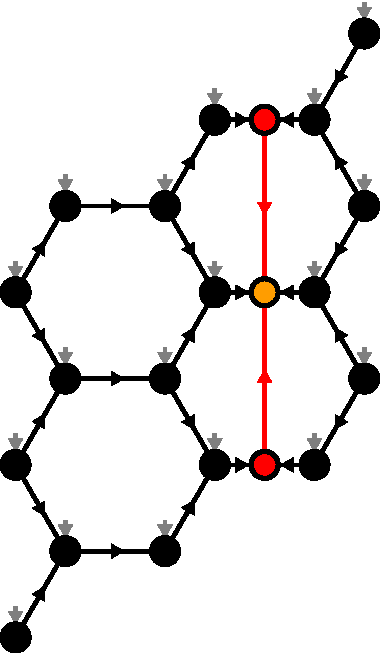
\includegraphics[scale=0.5]{figures/tikz/TFI/hexagonal_lattice/hexagonal_lattice_structure.pdf}
		}
	\end{minipage}
	\caption{In this figure we show imaginary TEBD results using disoTPS on the honeycomb lattice. We used two different values for the horizontal bond dimension, $D_\text{horizontal} = D$ and $D_\text{horizontal} = D^2$. The bond dimension along the orthogonality hypersurface was chosen as $\chi = 6\cdot D$. For the YB move we used the approximate Rényi-$0.5$ disentangler with a maximum of $N_\text{iter} = 100$ iterations per YB move. The model is the TFI model on a $4\times 4$ honeycomb lattice at a transverse field of $g = 3.5$. On the right we show the disoTPS structure of a $3\times 3$ honeycomb lattice as comparison.}
	\label{fig:tfi_gs_energy_vs_dtau_honeycomb}
\end{figure}